% ****** Start of file apssamp.tex ******
%
%   This file is part of the APS files in the REVTeX 4.2 distribution.
%   Version 4.2a of REVTeX, December 2014
%
%   Copyright (c) 2014 The American Physical Society.
%
%   See the REVTeX 4 README file for restrictions and more information.
%
% TeX'ing this file requires that you have AMS-LaTeX 2.0 installed
% as well as the rest of the prerequisites for REVTeX 4.2
%
% See the REVTeX 4 README file
% It also requires running BibTeX. The commands are as follows:
%
%  1)  latex apssamp.tex
%  2)  bibtex apssamp
%  3)  latex apssamp.tex
%  4)  latex apssamp.tex
%
\documentclass[%
% reprint,
%superscriptaddress,
%groupedaddress,
%unsortedaddress,
%runinaddress,
%frontmatterverbose, 
preprint,
%preprintnumbers,
%nofootinbib,
%nobibnotes,
%bibnotes,
 amsmath,amssymb,
 aps,
%pra,
%prb,
%rmp,
%prstab,
%prstper,
%floatfix,
]{revtex4-2}

\usepackage{graphicx}% Include figure files
\usepackage{dcolumn}% Align table columns on decimal point
\usepackage{bm}% bold math
%\usepackage{hyperref}% add hypertext capabilities
%\usepackage[mathlines]{lineno}% Enable numbering of text and display math
%\linenumbers\relax % Commence numbering lines

%\usepackage[showframe,%Uncomment any one of the following lines to test 
%%scale=0.7, marginratio={1:1, 2:3}, ignoreall,% default settings
%%text={7in,10in},centering,
%%margin=1.5in,
%%total={6.5in,8.75in}, top=1.2in, left=0.9in, includefoot,
%%height=10in,a5paper,hmargin={3cm,0.8in},
%]{geometry}

\begin{document}

\preprint{}

\title{Heart stroke-volume variability in a murine model for heart failure with reduced ejection fraction}% Force line breaks with \\
%\thanks{A footnote to the article title}%

\author{Gemma Fernández-Mendoza}
 \email{gemmag.fernandez@gmail.com}
\affiliation{%
 Departamento de Física, Escuela Superior de Física y Matemáticas, Instituto Politécnico Nacional, 07738 Ciudad de México, México
}%

\author{Moisés Santillán}
 \homepage{http://moises-santillan.github.io}
 \email{msantillan@cinvestav.mx}
\affiliation{
 Centro de Investigación y de Estudios Avanzados, Unidad Monterrey, 66628 Apodaca NL, México
}%

\date{\today}% It is always \today, today,
             %  but any date may be explicitly specified

\begin{abstract}
Write an abstract
\end{abstract}

%\keywords{Suggested keywords}%Use showkeys class option if keyword
                              %display desired
\maketitle

%\tableofcontents

\section{\label{sec:intro}Introduction}

\section{Materials and Methods}

\section{Results}

\subsection{Experimental and heart variability analysis}

According to the procedures outlined in Section Materials and Methods, we conducted the experiments on the control and experimental groups. We were able to calculate the heart's left ventricle volume as a function of time using the recorded data. This, along with the data on the ventricle pressure that was also recorded, made it possible to reconstruct for each experimental record the so-called P-V diagrams illustrated in Fig. XXX. Thereafter, we were able to extract time series of physiological interest from these diagrams, such as those of successive cardiac-cycle periods and stroke volumes.

We took the time series of consecutive cardiac-cycle periods and calculated the mean cycle duration for each experimental record, then averaged all of the values obtained in each group. Figure \ref{fig:fig01} depicts the obtained results. No significative difference can be appreciated between the results of the control group and those of the group of mice with induced cardiac failure. This finding contradicts the findings of \citet{Kamen_1995}, who found that the heart rate increases in patients with chronic heart failure. However, we must remember that the sympathetic and parasympathetic nervous systems regulate heart rate. As a result, the fact that mice were anesthetized in our experimental protocol, which affected such pathways, may explain the observed results.

\begin{figure}[h!]
    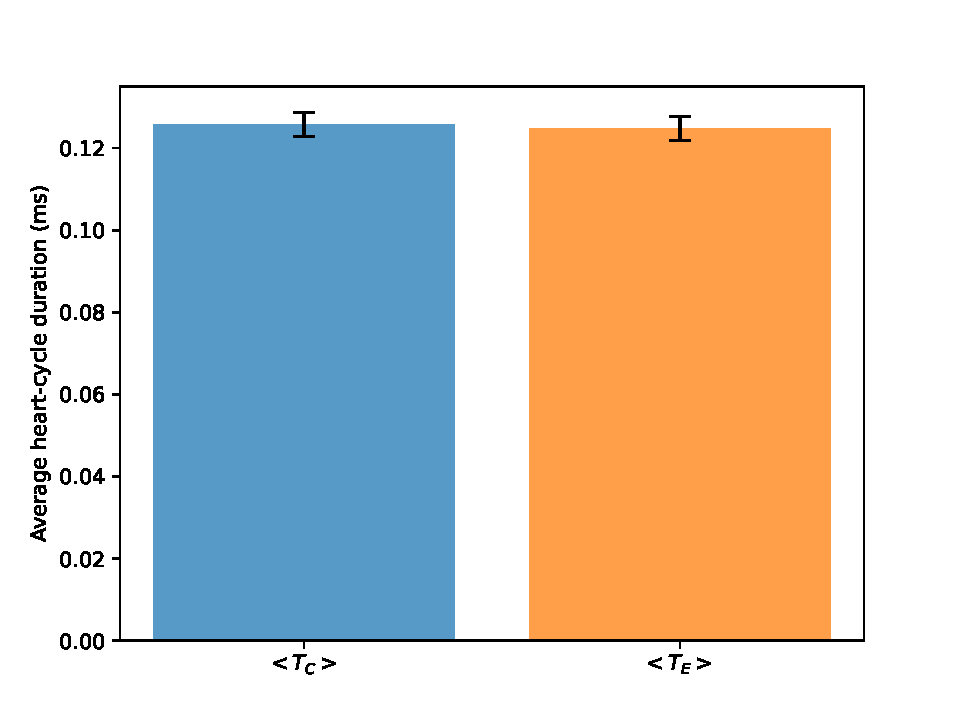
\includegraphics[width=3in]{Fig01.pdf}
    \caption{Average cardiac-cycle periods for control and experimental groups}
    \label{fig:fig01}
\end{figure}

We also calculated the mean values for the time series of consecutive stroke volumes for every experimental record. Then we averaged the results from each group and plotted the results in Fig. \ref{fig:fig02}. As expected, there is a significant reduction in stroke volume in the group with induced heart failure when compared to the control group.

\begin{figure}[h!]
    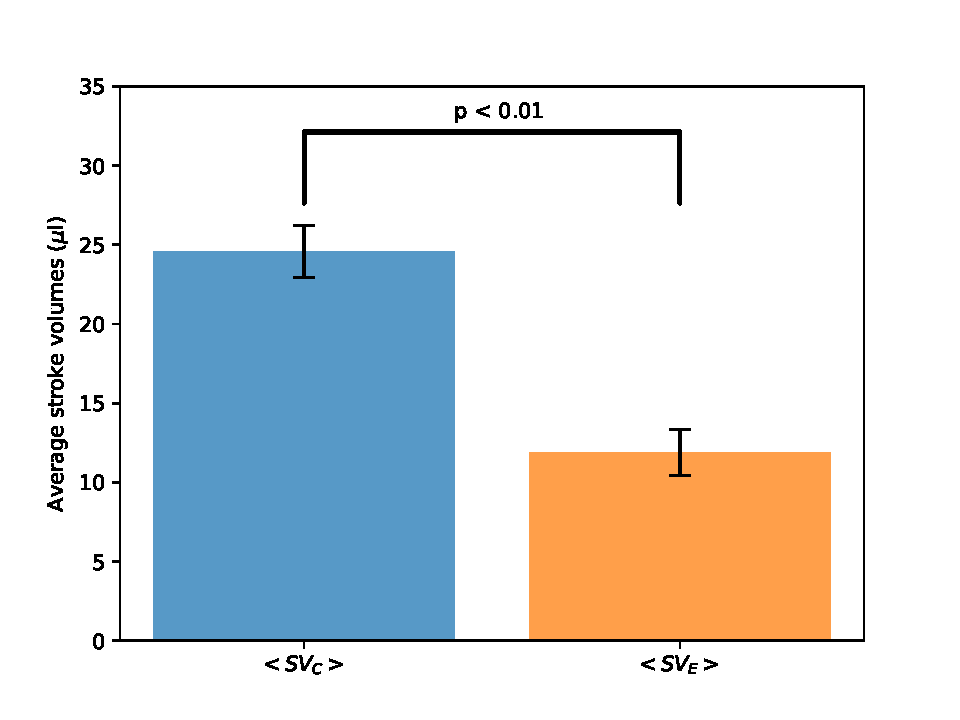
\includegraphics[width=3in]{Fig02.pdf}
    \caption{Average stroke volumes for control and experimental groups}
    \label{fig:fig02}
\end{figure}

We were interested in studying the variability of heart-cycle periods and stroke volumes. In this regard, a variety of techniques have been used to measure heart rate variability. The vast majority of them are founded on the concept of signal stationarity. However, the heart rate's inherent non-stationary nature---which undergoes continuous physiological change to adapt to external stimuli---presents a significant challenge that could result in inaccurate results \citep{Marwan_2007}. Although several signal preprocessing methodologies have been proposed to address these issues, nonlinear analysis-based strategies are commonly employed and appear to produce reliable results. \citep{Marwan_2002, Aubert_2003, Marwan_2007, Giuliani_1998, Rajendra_Acharya_2006, Webber_1994, Henriques_2020}. One of them that is used in different scientific domains is the Poincairé plot \citep{Hoshi_2016, Webber_1994, Voss_2008}. In a Poincairé plot, all values in a time series are plotted against previous values, resulting in an ellipsoidal point cloud. The standard deviations of the point projections along the lines $y = x$ (SD2) and $y = -x$ (SD1) can be used to quantitatively analyze this diagram. The transverse axis of the ellipse (SD1) is a measure of the short-term changes in the the time series, while the longitudinal axis (SD2) reflects long-term changes. In the particular case of heart-beat duration time-series, SD1 is considered as an indicator of the parasympathetic activity, whereas SD2 is considered as an inverse indicator of the sympathetic activity \citep{Zimatore_2022}.

We measured the above described Poincaré-plot indices of heart-cycle period variability for every experimental record, and averaged the results corresponding the the control and experimental groups. The outcomes are plotted in Fig. \ref{fig:fig03}. Observe that no statistically significative difference exists between the indices corresponding to the control and experimental groups. This suggests that, under our experimental conditions, heart failure does not affect heart rate variability (HRV). This finding contradicts \citet{Kamen_1995} and other authors, who have reported that HRV decreases in patients with hart failure and we believe that it is also related to the fact that mice are anesthetized in our experimental protocol. Recall the anesthesia affects the sympathetic and parasympathetic pathways and that they, in turn, influence heart rate variability.

\begin{figure}[h!]
    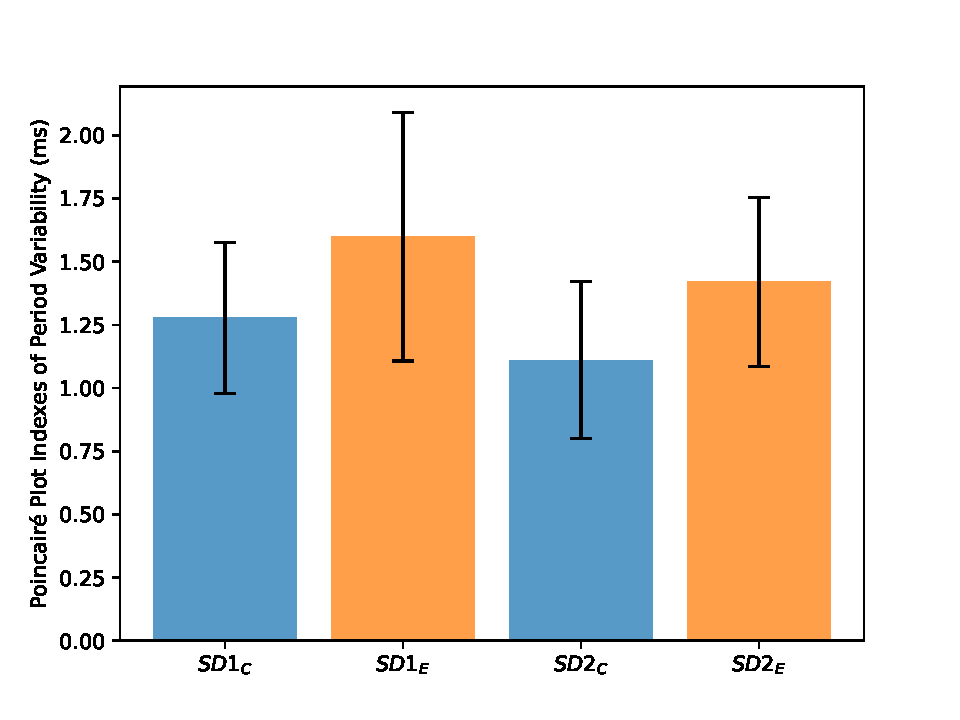
\includegraphics[width=3in]{Fig03.pdf}
    \caption{}
    \label{fig:fig03}
\end{figure}

The same methodology was used to investigate the variability of stroke volumes. The results are shown in Fig. \ref{fig:fig04}. The experimental group's SD1 and SD2 values are significantly lower than those of the control group. This suggests that heart failure affects the mechanisms in charge of controlling stroke volume. Furthermore, the absence of changes in HRV suggests that both types of variability are dissociated.
\begin{figure}[h!]
    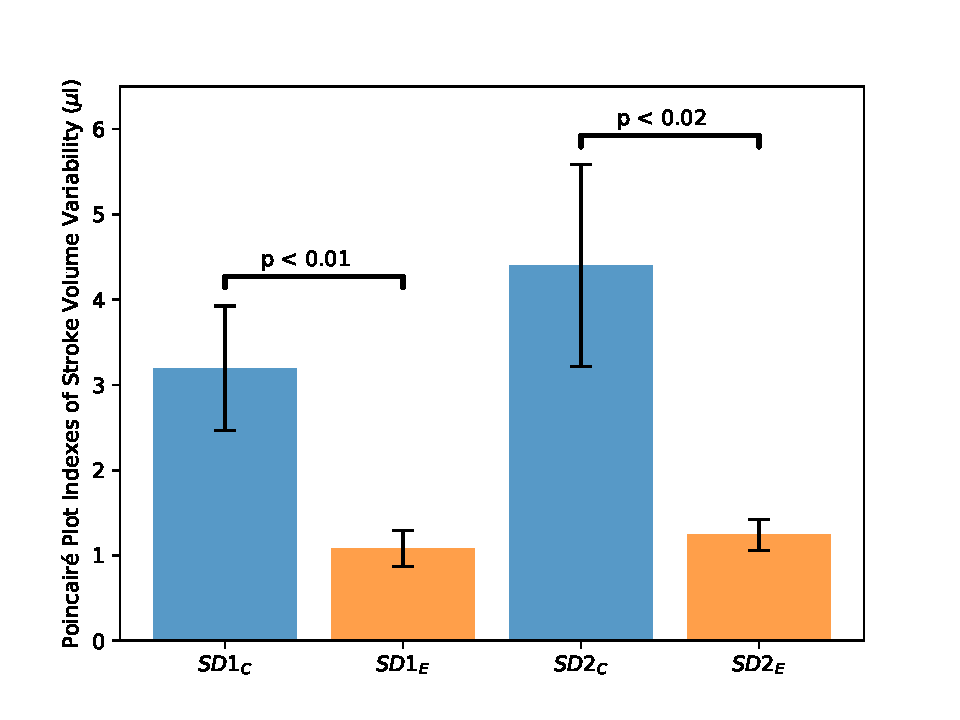
\includegraphics[width=3in]{Fig04.pdf}
    \caption{}
    \label{fig:fig04}
\end{figure}

\subsection{Mathematical Model}

\begin{figure}
\includegraphics[width=4in]{model.pdf}
\caption{Schematic representation of the model}
\label{fig:model}
\end{figure}

\section{Concluding Remarks}

\begin{acknowledgments}
We wish to acknowledge the support of the author community in using
REV\TeX{}, offering suggestions and encouragement, testing new versions,
\dots.
\end{acknowledgments}



\bibliography{manuscript}% Produces the bibliography via BibTeX.

\end{document}
%
% ****** End of file apssamp.tex ******
